\documentclass{article}
\usepackage[utf8]{inputenc}
\title{Evaluación 2}
\author{Roberto Alexis Gómez Pintor}
\usepackage{float}
\usepackage{graphicx}
\begin{document}
\maketitle
\section{Introduccion.}
El sistema de Lorenz es un sistema de ecuaciones diferenciales ordinarias estudiadas por primera vez por Edward Lorenz. Es notable por tener soluciones caóticas para ciertos valores de parámetros y condiciones iniciales. En particular, el atractor de Lorenz es un conjunto de soluciones caóticas del sistema Lorenz que, cuando se trazan, se asemejan a una mariposa o al ocho.
\section{Desarrollo}
En la evaluación se desarrollo 2 códigos referente al sistema de Lorenz, uno generaba una animación(archivo tipo gif) y uno visual(imágenes estáticas). A partir de estos 2 archivos generamos cambios para modificar los valores de beta, rho y sigma. Ademas se construyo una gráfica bidimensional de las soluciones x(t),y(t),z(t) para observar la evolución temporal.
\section{Resultados}
Ya obtenido la información generamos imágenes en movimientos del sistema de lorenz con diferentes valores, por desgracia cada imagen de movimiento genero una aproximación de 300 imágenes sin movimiento que genero fuera difícil subir los archivos al repositorio de trabajo, así que solo usaremos las obtenidas en los archivos visuales y no los animados.
\section{Gráficas}
\begin{figure}[!ht]
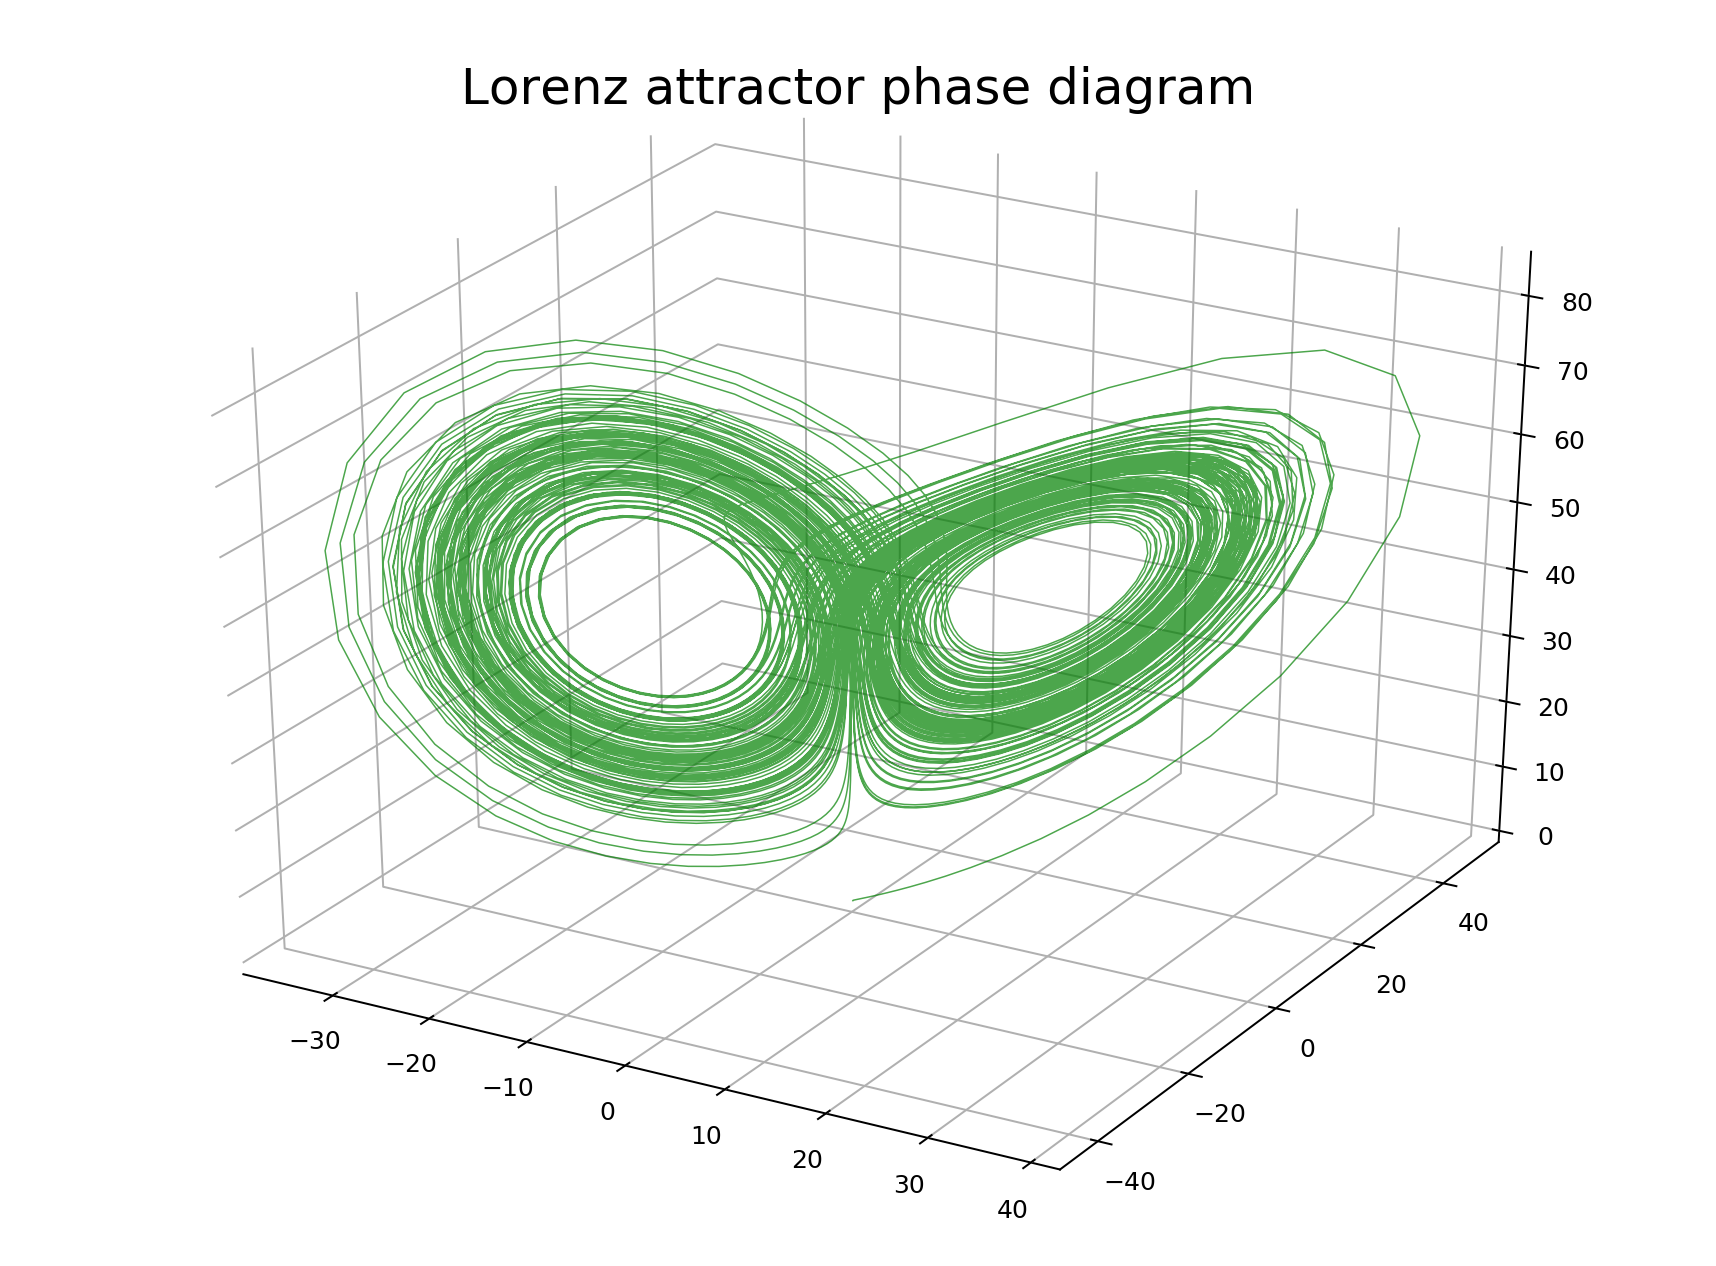
\includegraphics[width=\linewidth]{lorenz2-attractor-3d.png}
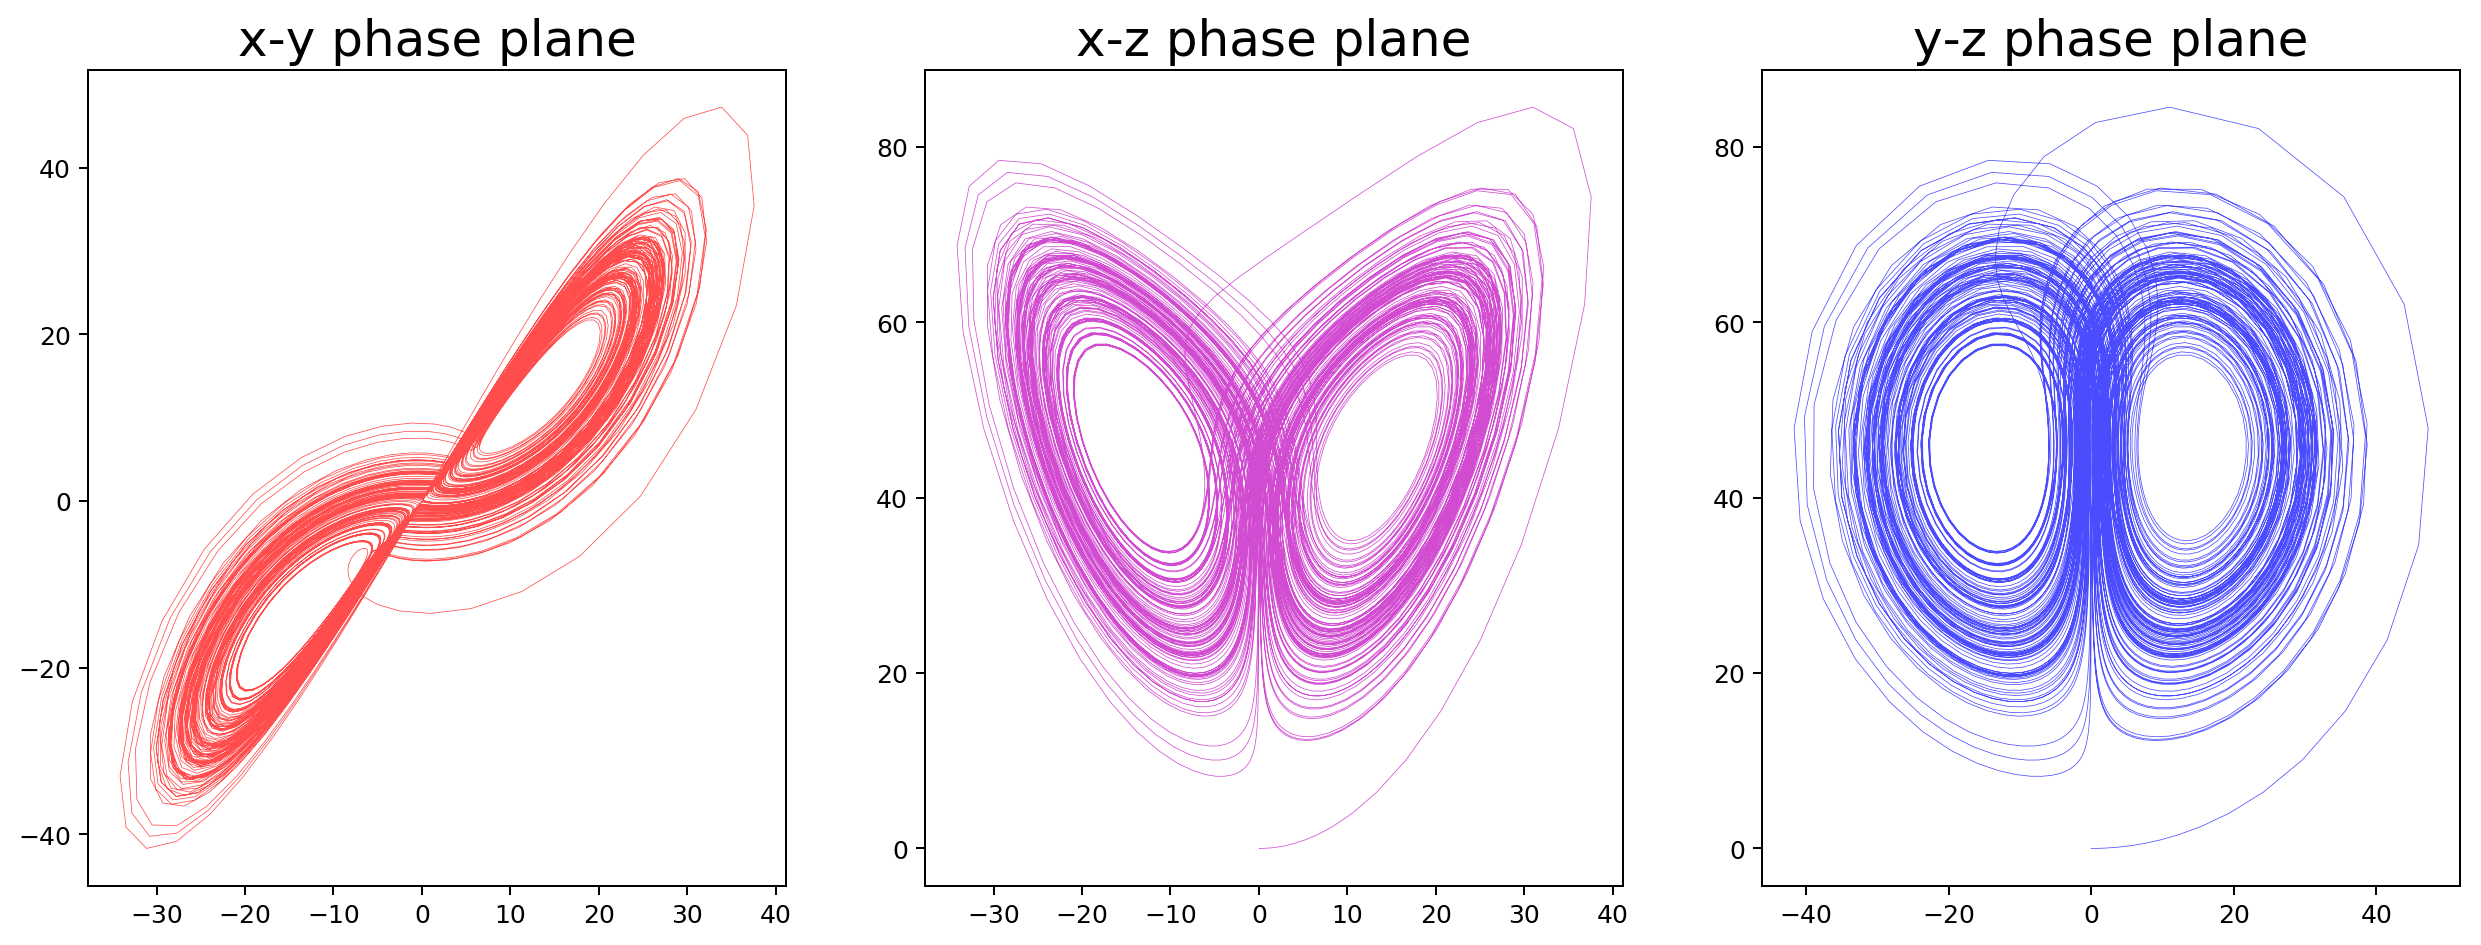
\includegraphics[width=\linewidth]{lorenz2-attractor-phase-plane.png}
\end{figure}
\begin{figure}[!ht]
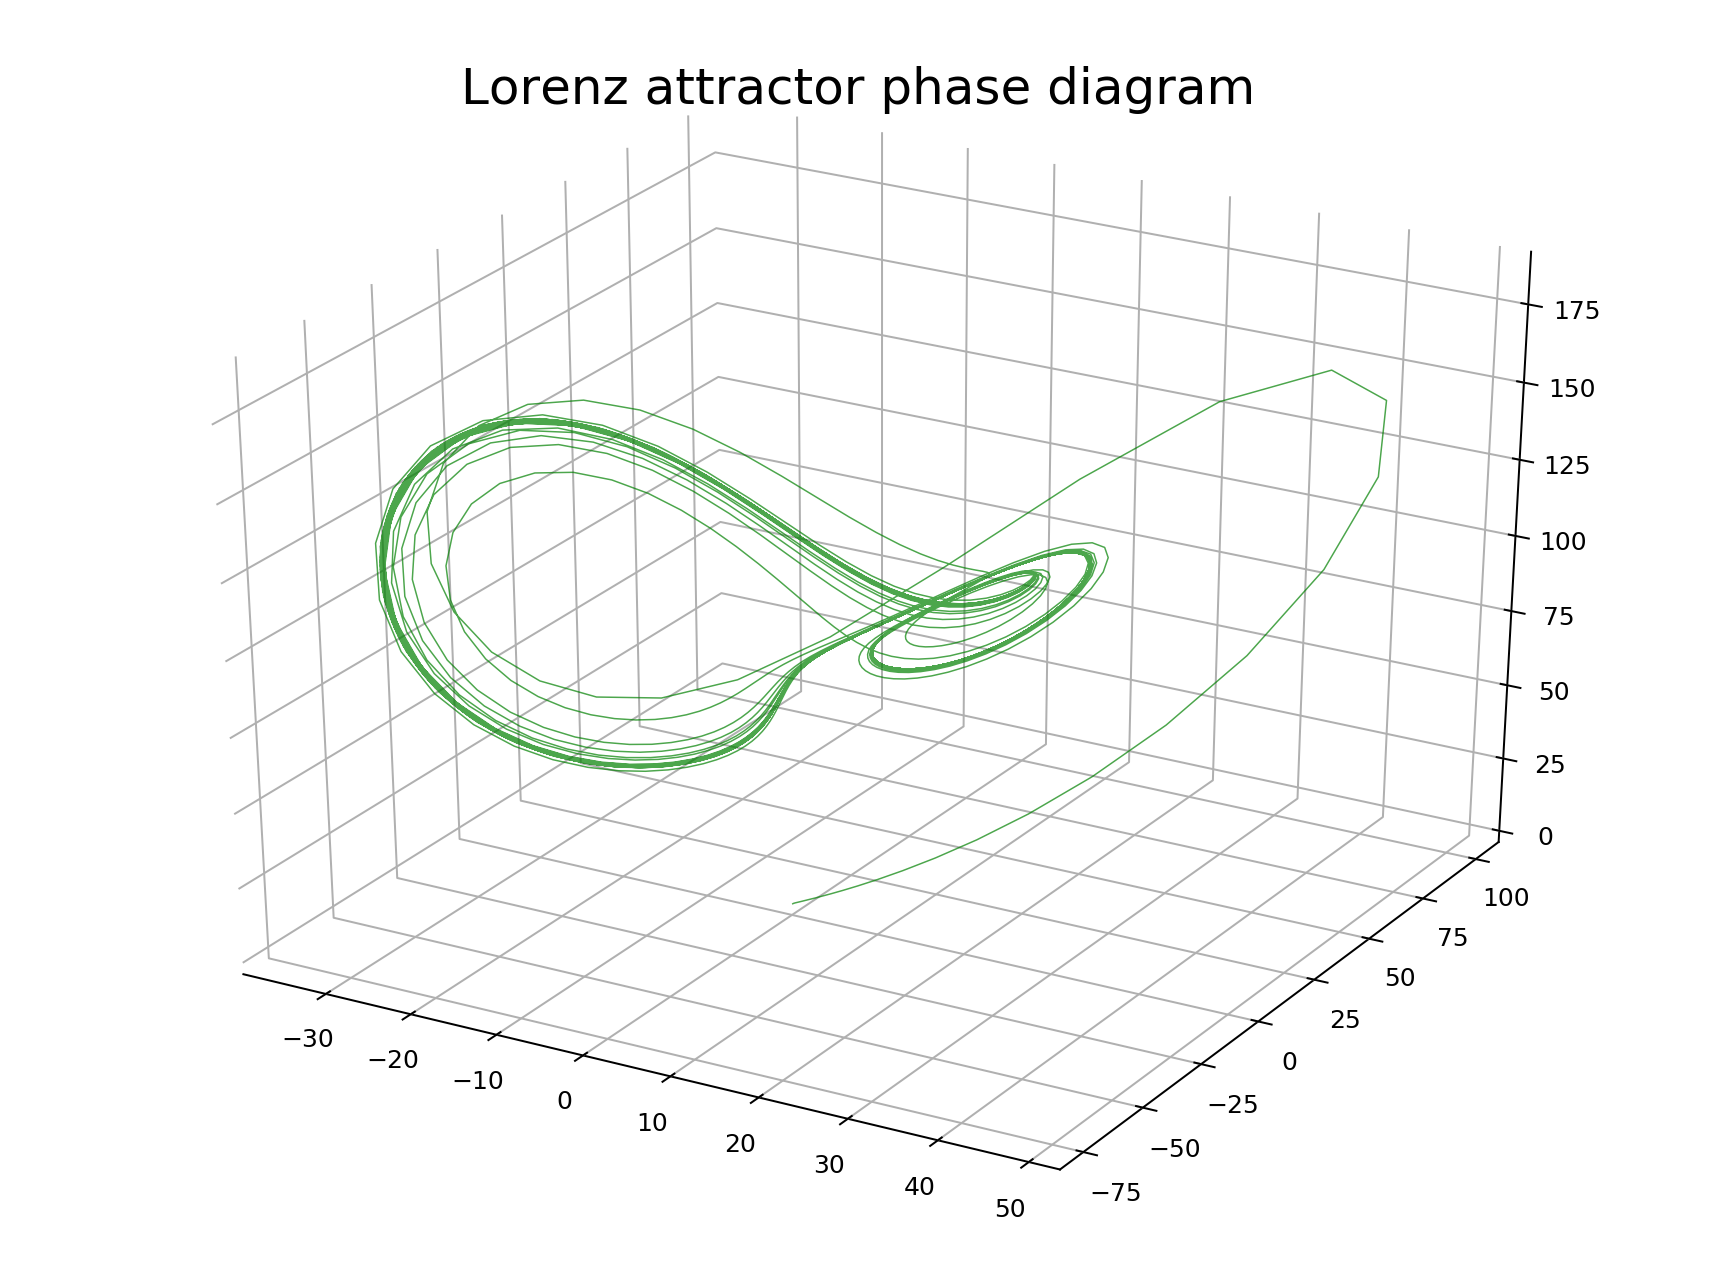
\includegraphics[width=\linewidth]{lorenz3-attractor-3d.png}
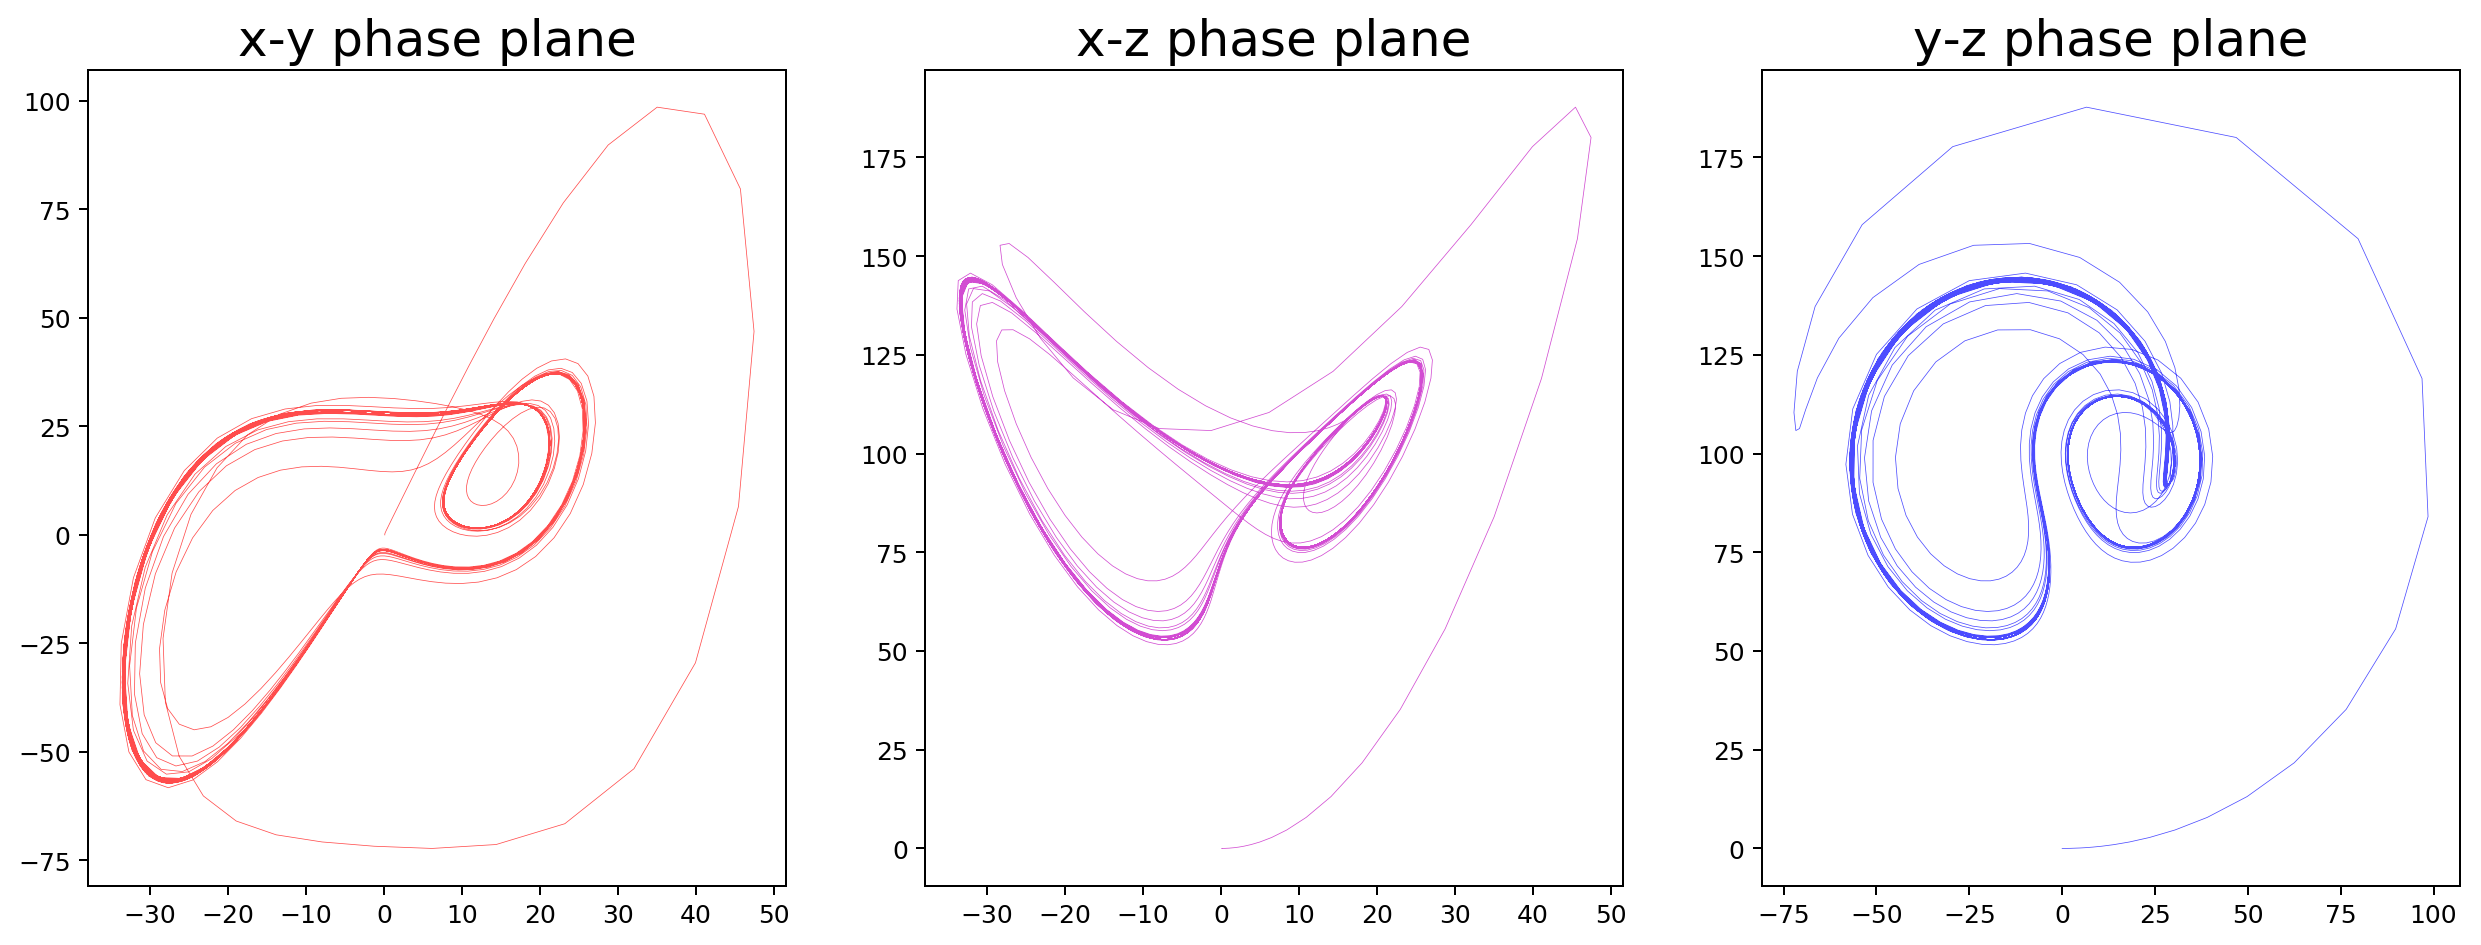
\includegraphics[width=\linewidth]{lorenz3-attractor-phase-plane.png}
\end{figure}
\end{document}